\chapter{Umsetzung - Irena Bala}
\section{Allgemeine Beschreibungen}
Bei dieser Diplomarbeit wurde darauf abgezielt, ein intelligentes System zu entwickeln, dass die täglichen Aufgaben des Menschen erleichtert und so viel wie möglich automatisch gesteuert wird. Um dieses Ziel zu erreichen wurden bestimmte Komponenten im System implementiert. Diese wurden mit Absicht so ausgewählt, um die zukünftige Erweiterung und Umsetzung des Projekts auf vielen Anwendungsgebiete zu erlauben.  Ein weiterer Zweck besteht also darin, das System zu vervollständigen und sein Entwicklungsgemeinde zu vergrößern. \\
Diese Komponente wurden in unterschiedlichen Bereichen unterteilt. Der erste Bereich ist die Datenbank. Die Datenbank ist der wesentliche Bestandteil des Systems, weil die Basis für die Speicherung der benötigten Daten bildet. In die Datenbank wurden alle von den verwendeten APIs gekommene Daten gespeichert. Außerdem wurden dort auch die Schuldaten gelegen. Diese Daten sind ein separater Teil des Projekts, die in den folgenden Kapiteln genauer erklärt werden. \\
Die Darstellung an Bildschirm von den gespeicherten Daten wurde durch eine Admin-Webseite realisiert. Es wurden viele Layouts für die Anzeige (Bildschirm) entworfen, damit die Informationen auf unterschiedlichen Weisen dargestellt werden. \\
Das Infotainment System funktioniert wie die meisten Systeme nach dem Server- Client Prinzip. Sowohl der Server, als auch der Client werden näher betrachtet, denn sie die Hauptbereiche des ganzen Systems sind. 
Ein weiterer interessanter Bereich ist der Chatbot. Chatbot wurde deswegen implementiert, weil es die Interaktion des Menschen mit dem System ermöglicht und dadurch wurde angenommen, dass die Umsetzung dieses Komponentes das Interesse des Menschen an dem System erhöhen wird. \\
Dies war eine allgemeine Beschreibung von den bis jetzige erreichte Ergebnisse. Entsprechend der jeweiligen Arbeitsaufteilung werden in den folgenden Kapiteln einige von den oben genannten Aspekten näher erläutert. \\
\subsection{Chatbot} 
In diesem Unterkapitel wird eine Einführung in Chatbot gemacht und dessen Umsetzung erklärt.
\subsubsection{Einführung in Chatbot}
Chatbot ist ein sehr wichtiger Komponent von der künstlichen Intelligenz. Es bietet eine Kommunikationsschnittstelle zwischen Menschen und technischen Systeme. Chatbot empfängt Anweisungen in Textform von den Menschen und überträgt diese so, dass die Systeme diesen Anweisungen entsprechen. Basierend auf was Chatbots anbieten, werden als sehr schlaue Komponente angesehen, die immer mehr implementiert werden.\cite{einstein,knuthwebsite}
\subsubsection{Umsetzung von Chatbot}
Chatbot wurde bei dieser Diplomarbeit so implementiert, dass es den Schülern die Möglichkeit gibt, aufgenommene Bilder zum Chatbot zu schicken und dann diese Bilder werden automatisch auf dem Bildschirm angezeigt. Das ist auch die wesentliche Funktionalität von Chatbot bei diesem Projekt. \\
Um den Chatbot zu implementieren, haben viele kleine Prozesse stattgefunden, die als weitere oder zusätzliche Funktionen angesehen werden können.\\
Zuerst wurde Telegram Bot API als eine Schnittstelle für die Chatbot-Implementierung ausgewählt. Durch diese API können neue Bots erstellt, bearbeitet und verändert werden. Telegram Bot API funktioniert gleich wie die anderen Kommunikationsapplikation z.B Whatsapp. Der wesentliche Unterschied ist, dass bei dieser Applikation wird nicht nur die Möglichkeit mit anderen Menschen zu chatten angeboten, sondern auch mit Chatbots. Jedes Bot, das erstellt wird, bekommt ein Token, dass eindeutig für das Bot ist, wie die Telefonnummer für uns eindeutig ist. \\
Die komplette Funktionalität des Bots wurde in RaspberryPI Server, mithilfe der Python Programmiersprache programmiert. \\
Je nachdem ob die Person, die mit dem Bot chatten will, als ein normaler Benutzer oder ein Administrator in der Datenbank definiert ist, werden ihm verschiedene Funktionen im Zusammenhang mit dem Bot zur Verfügung gestellt. Die Nachrichten, die zu dem Bot geschickt werden, werden nach Inhalt überprüft. Basierend auf Inhalt der Nachrichten, wird der Bot auf verschiedene Weisen reagieren.\\
Die Art der Umsetzung bzw. Realisierung aller diesen Funktionen kann im Unterkapitel 2.1 gelesen werden.   

\subsection{Server}
Das Infotainment System wie die anderen technischen Systeme, funktioniert nach dem Client-Server Prinzip. Das bedeutet, es gibt einen Server und einen Client, die miteinander kommunizieren. Der Client ist in diesem Projekt die Anzeige bzw. das Bildschirm, dass die von dem Server bekommene Daten darstellt. \\
Im Server liegen aber alle benötigten Informationen für die Darstellung. Diese Informationen sind auf der Datenbank gespeichert, die auf dem Server stattfindet.\\
Der Server beinhaltet auch die grundlegenden Skripts für die Chatbot-Implementierung und für die Programmierung der Admin-Webseite. Im Server wurde auch das SSL Zertifikat für eine sichere Datenübertragung erstellt.\\
Die Kommunikation zwischen dem Client und dem Server wird dann aufgebaut, wenn Daten von dem Server ausgewählt und zum Client geschickt werden. 
Der Server ist der grundlegende Teil des Projekts. Es enthält alle benötigten Ressourcen für die vollständige Umsetzung des Systems.
\subsection{Technologien}
In diesem Unterkapitel werden die verwendeten Technologien und Software-Ressourcen beschrieben.  Es werden die grundlegenden Theorien, die hinter diesen Technologien stehen, im Detail erläutert. Dazu werden auch die Gründe für die Auswahl der Software-Ressourcen erklärt. 
Die unterliegende Tabelle listet die verwendeten Technologien auf und daneben steht auch eine kurze Beschreibung für jede Technologie.
\begin{table}[h]
	\begin{center}

\label{tab:Tabelle1}
\resizebox{\textwidth}{!}{
	\begin{tabular}{ | l |l |p{5cm} |} 
		\hline
		\textbf{Name} & \textbf{Beschreibung}\\
		\hline
		Apache HTTP Server & Webserver   \\ \hline
	    MySQL& Relationales Datenbanksystem\\ \hline
		PHP	& Serverseitige Programmiersprache\\ \hline
		JavaScript & Programmiersprache zur dynamischen 
		Veränderung von Webseiten \\ \hline 
		Python	& Objektorientierte/ prozedurale Programmiersprache \\ \hline
		HTML &	Auszeichnungssprache zur Erstellung von Inhalten bei Webseiten \\ \hline
		CSS	& Methode, zur Entkopplung von Designanweisungen einer HTML Datei \\ \hline
		Wetter API &	Schnittstelle zur Aufnahme von Wetterdaten aus großen Wettervorhersage-Datenbanken \\ \hline
		JSON	& strukturiertes Dateiformat \\ \hline 
		Telegram API &	Schnittstelle zur Implementierung von Chatbot \\ \hline
		Raspberry PI &	Minirechner, der für Scripting, Linux Programmierung geeignet ist \\ \hline
		SSL &	Methode zur verschlüsselten Datenübertragung zwischen Browser und Server \\ \hline
		
\end{tabular} }
%\end{adjustbox} 
\caption{Technologien}
\end{center}
\end{table} 
\subsubsection{Was ist Apache HTTP Server?} 
Der Apache HTTP\footnote{Hypertext Transfer Protocol}\nomenclature{HTTP}{Hypertext Transfer Protocol} Server ist ein weltweit verbreitender Web Server. Dieser Server ist Open Source, das bedeutet, dass es keine Lizenz gekauft werden soll, um es zu verwenden. Es ist kompatibel auf allen kohärenteren Betriebssystemen, beispielsweise Linux, Windows, Mac OS und andere. Es bietet viele Versionen an, die zu unterschiedlichen Anwendungsgebiete passen und verbesserte Eigenschaften bereitstellen. Durch dieses Webservers können Webseiten erstellt werden. Die Erstellung der Webseiten erfolgt über serverseitige Scriptsprachen, die von dem Server selbst nicht unterstützt werden. Sie werden als Zusatzfunktionen angehängt. \\
Der Apache HTTP Server bietet viele Funktionalitäten an, die seine Entwicklungsumgebung vergrößern. Die wichtigste davon ist die Möglichkeit der Integration eines SSL \footnote{Secure Socket Layer}\nomenclature{HTTP}{Secure Socket Layer}Zertifikats. Das ermöglicht die Übertragung der Daten in einer verschlüsselten Form. Die detaillierte Funktionsweise eines SSL Zertifikats wird in den Unterkapiteln beschrieben.  \cite{50_apache}
\subsubsection{Funktionsweise von Apache HTTP Server} 
„Obwohl Apache als Webserver bezeichnet wird, handelt es sich nicht um einen physischen Server. Apache ist eine Software, die auf einem Server ausgeführt wird. Seine Aufgabe ist es, eine Verbindung zwischen einem physischen Server mit den gespeicherten Webseiten und den Browsern der Internetuser herzustellen. \\
Wenn ein User eine URL in seinen Webbrowser eingibt, sendet der Browser eine HTTP oder HTTPS \footnote{Hypertext Transfer Protocol Secure}\nomenclature{HTTPS}{Hypertext Transfer Protocol Secure} Anforderung an den Server, auf dem die Webseite gespeichert ist.“ \cite{50_apache} \\
\\

\subsubsection{Was ist MySQL?} 
MySQL ist ein weitverbreitetes relationales Datenbanksystem. Die Datenbanksysteme werden allgemein zur Datenspeicherung und Datenverwaltung verwendet. Ein wichtiges Kriterium für die Datenspeicherung ist die Performanz. Diese Anforderung wird durch MySQL optimal erfüllt. Das ist auch der Grund, warum dieses Datenbanksystem so populär und bekannt ist. Die von MySQL für die Abarbeitung, Verwaltung und Systematisierung von Daten verwendete Sprache ist SQL\footnote{Structured Query Languague}\nomenclature{SQL}{Structured Query Language}. MySQL ist auch eine Open Source Software,
die in meisten Fällen in Verbindung mit serverseitigen Scriptsprachen wie PHP, vorkommt. \cite{50_mysql}
\subsubsection{Funktionsweise von MySQL} 
Das MySQL Datenbanksystem wird sehr häufig implementiert. Es gibt viele Unternehmen und Institutionen, die ihre Daten über eine gewisse Zeit speichern wollen. Das MySQL Datenbanksystem, das die Daten beinhaltet, wird als ein Server vorgesehen. Jeder, der versucht, Zugriff auf diese Daten zu haben, wird als ein Client vorgesehen. Der Server kann die erforderliche Zugänglichkeit erlauben oder nicht. Das hängt von den Clientrechten ab. Die Daten können von den Clients selektiert, bearbeitet oder gelöscht werden. Diese Ereignisse erfolgen durch SQL-Abfragen. Die SQL-Abfragen werden mithilfe der SQL Datenbanksprache erstellt. \cite{50_mysql}
\subsubsection{Was ist PHP?} 
PHP\footnote{Parallel History Project}\nomenclature{PHP}{Parallel History Project} ist eine serverseitige Programmiersprache. Das bedeutet, dass diese Sprache, um 
die vom Server auszuführenden Ereignissen zu programmieren, verwendet wird. 
PHP ist eine sehr verbreitete Programmiersprache, die am meisten zur Erstellung und Programmierung von Webseiten verwendet wird. Eigentlich ist PHP sehr flexibel, denn es einen großen Schnittstellenansatz anbietet.  Diese Programmiersprache kann auch im Zusammenhang mit Datenbanken genutzt werden. \cite{50_php}
\subsubsection{Funktionsweise von PHP} 
Hier kommt das Client-Server Prinzip wieder vor. Der Webbrowser ist der Client und der Webserver ist der Server. Der mit PHP programmiertes Skript wird zum Webserver geschickt, danach erfolgt die Rückgabe einer HTML-Datei als Antwort zum Webbrowser, der in diesem Fall als Client betrachtet wird. \cite{50_php}
\subsubsection{Was ist JavaScript?} 
JavaScript ist eine Programmiersprache, die am meisten zur Erstellung von dynamischen Funktionalitäten bei Webseiten, verwendet wird. Die JavaScript Programmiersprache hat in der Vergangenheit nur eine beschränkte Anzahl von Funktionen angeboten, aber heutzutage bietet sie eine Vielzahl von Einsatzmöglichkeiten. \cite{50_javascript}
\subsubsection{Mögliche Funktionen von JavaScript} 
„JavaScript wurde entwickelt, um dynamische HTML-Seiten per Webbrowser anzuzeigen. Die Verarbeitung von JavaScript erfolgt meist clientseitig direkt durch den Webbrowser. \\
Mit Hilfe der Skriptsprache JavaScript lassen sich viele dynamische Funktionen realisieren. Hier sind einige Beispiele für die Verwendung von JavaScript:
\begin{itemize}
	\item  dynamische Veränderung von Webseiten – zum Beispiel für die Anzeige eines formatierten und aktualisierten Datums
\end{itemize}
\begin{itemize}
	\item Prüfung von in Formularen eingegebenen Daten auf Plausibilität
\end{itemize}
\begin{itemize}
	\item Anzeige von Laufschriften oder Bannern
\end{itemize}
\begin{itemize}
	\item 	Öffnen und Anzeigen von Dialogfenstern
\end{itemize}
\begin{itemize}
	\item Aktualisieren von Daten einer Webseite ohne neu laden im Browser
\end{itemize}
\begin{itemize}
	\item 	Unterstützung der Eingabe von Daten durch den User
\end{itemize}
\begin{itemize}
	\item Veränderung von Texten oder Grafiken durch den Mauszeiger" \cite{50_javascript}
\end{itemize}
\subsubsection{Was ist Python?} 
Python ist eine objektorientierte Programmiersprache, aber kann auch in prozedurale Programmierung verwendet werden. Sie wurde ausschließlich zum Zweck der einfach einprägsamen Syntax entwickelt. Andererseits haben die Entwickler der Systematisierung des Codes große Bedeutung beigemessen. Wegen dieser angewandten Eigenschaften kann Python in die Gruppe der leichten Programmiersprachen aufgenommen werden. Diese Programmiersprache wird viel verwendet, aber was die Anwendungsumgebung besonders erhöht, ist die Möglichkeit andere Module anzuhängen. Es ist auch eine Open Source Software, der von den Programmierern verwendet, verändert, angepasst bzw. bearbeitet werden kann. Es wird meistens für komplexe Aufgaben verwendet werden, deswegen wird es als eine Hochsprache betrachtet. \cite{50_python}
\subsubsection{Merkmale von Python} 
\begin{itemize}
	\item Einfach einprägsame Syntax
\end{itemize}
\begin{itemize}
	\item Objektorientierte und prozedurale Programmiersprache
\end{itemize}
\begin{itemize}
	\item Open Source 
\end{itemize}
\begin{itemize}
	\item Hoches Niveau Programmiersprache
\end{itemize}
\begin{itemize}
	\item Leicht veränderbare Programmiersprache\cite{50_python}
\end{itemize}
\subsubsection{Was ist HTML?} 
HTML\footnote{HyperText Markup Language}\nomenclature{HTML}{HyperText Markup Language} ist keine Programmiersprache, die wird für die Erstellung von Inhalten bei Webseiten verwendet. Diese Inhalte können Texte, Bilder oder andere Komponente sein. HTML wird als eine Auszeichnungssprache betrachtet. Sie ist nicht nur für die Erstellung von Webseite-Inhalten zuständig, sondern auch für ihr Design. Diese Sprache liegt mithilfe von bestimmten Tags die Struktur einer Webseite fest. Im Tag werden die Inhalte gespeichert. Es gibt bestimmte Tags für verschiedene Layout-Elemente.\cite{50_html} %\cite{einstein}
\subsubsection{Was ist CSS?} 
CSS\footnote{Cascading Style Sheets}\nomenclature{CSS}{Cascading Style Sheets} wird im Zusammenhang mit HTML verwendet. Diese Methode wird unten genauer betrachtet. \\
„CSS steht für Cascading-Style-Sheets und ist eine Möglichkeit für HTML-Dokumente, den Inhalt einer Seite von den Designanweisungen der einzelnen Elemente, wie zum Beispiel Überschriften, Zitaten) zu entkoppeln.“ \cite{50_css}
\subsubsection{Was ist Raspberry PI?} 
Der Raspberry PI ist ein Minirechner, die zur Linux Programmierung, Shell Scripting und Realisierung von technischen Projekten verwendet wird. Es braucht eine Tastatur, eine Maus, ein Netzteil, VGA\footnote{Video Graphics Array}\nomenclature{VGA}{Video Graphics Array} und HDMI\footnote{High-Definition Multimedia Interface}\nomenclature{HDMI}{High-Definition Multimedia Interface}-VGA Konverter, damit es genutzt werden kann. Die Konfiguration von einem Raspberry PI erfolgt durch eine SD-Karte. Diese SD\footnote{Secure Digital Memory Card}\nomenclature{SD}{Secure Digital Memory Card}-Karte beinhaltet das Image, wo das Betriebssystem liegt. Ein Raspberry PI kann in Zusammenhang mit vielen anderen Komponenten verwendet werden.\cite{50_raspi}
\subsubsection{Was ist SSL?} 
SSL steht für Secure Socket Layer und ist für die verschlüsselte Übertragung der Daten vom Browser zum Server verantwortlich. Die Verbindung zwischen dem Server und dem Browser erfolgt durch das HTTPS Protokoll. Das ist ein Kommunikationsprotokoll, das eine verschlüsselte Datenübertragung ermöglicht. Heutzutage wird TLS\footnote{Transport Layer Security}\nomenclature{SD}{Transport Layer Security} am meisten verwendet, der der neueste und modernste Standard von SSL ist.\cite{50_ssl}
\subsubsection{SSL-Verschlüsselung}
Um eine verschlüsselte Verbindung zwischen einem Browser und einem Server aufzubauen, werden SSL – Zertifikaten integriert. Mittels ein SSL Zertifikats wird die Authentizität einer Webseite überprüft. Das SSL Zertifikat wird von einer Zertifizierungsstelle, erzeugt. Diese Zertifizierungsstelle heißt CA\footnote{Certificate Authority}\nomenclature{CA}{Certificate Authority} und erfordert einige Daten von dem Antragsteller, die für die Erstellung des Zertifikats notwendig sind. Als nächstes, erzeugt der Antragsteller für die Entschlüsselung und Verschlüsselung der zwischenübertragenen Daten ein öffentlicher, -und ein privater Schlüssel. Je grösser die Lange des Schlüssels ist, desto sicherer und besser ist. Meistens werden Schlüssel mit einer Länge von 256 Bit verwendet.\cite{50_ssl}
\subsubsection{Was ist Telegram Bot API?} 
Telegram Bot API\footnote{Application Programming Interface}\nomenclature{API}{Application Programming Interface} ist eine Schnittstelle, die die Implementierung von Chatbot ermöglicht. Es bietet verschiedene Funktionen an, nämlich die Einrichtung, Erstellung und die Verarbeitung von Bots. Diese Funktionen sind in der eigenen Dokumentation von Telegram Bot API klar beschrieben. \cite{50_telegram}  
\subsubsection{Was ist Wetter API?} 
„Wetter APIs sind Schnittstellen, die die Verbindung zu einer großen Wettervorhersage-Datenbank und die Aufnahme benötigter Daten ermöglichen.“ \cite{50_Wetter}
\subsubsection{Was ist JSON?} 
„JSON\footnote{JavaScript Object Notation}\nomenclature{JSON}{Javascript Object Notation} bietet einen einfachen Standard für die strukturierte Kodierung von Daten in Form von menschenlesbarem Text. Dies bietet Vorteile bei einer automatisierten Weiterverarbeitung, macht sie aber auch einer manuellen Inspektion und Überarbeitung besser zugänglich.“ \\ \cite{50_json}
\\
In der untenstehenden Tabelle sind alle Technologien zusammen mit dem Bereich wo sie gehören ersichtlich. 
\begin{table}[h]
	\begin{center}
		
		\label{tab:Tabelle1}
	
			\begin{tabular}{ | l |l |} 
				\hline
				\textbf{Bereich} & \textbf{Technologie}\\ \hline 
				Datenbank &	Apache HTTP Server, MySQL, PHP \\ \hline
				Anzeige &	HTML, CSS, JavaScript \\ \hline
				Server &	RaspberryPI, SSL \\ \hline
				Wetterdaten	 &Wetter API, JSON \\ \hline
				Chatbot &	Telegram API, Python \\ \hline
				
				\hline
				 
		
		\end{tabular} 
		\caption{Bereiche und Technologien}
	\end{center}
\end{table} 
\section{Technische Lösungen}
\subsection{Structured Software Design}
\begin{figure}[ht]	
	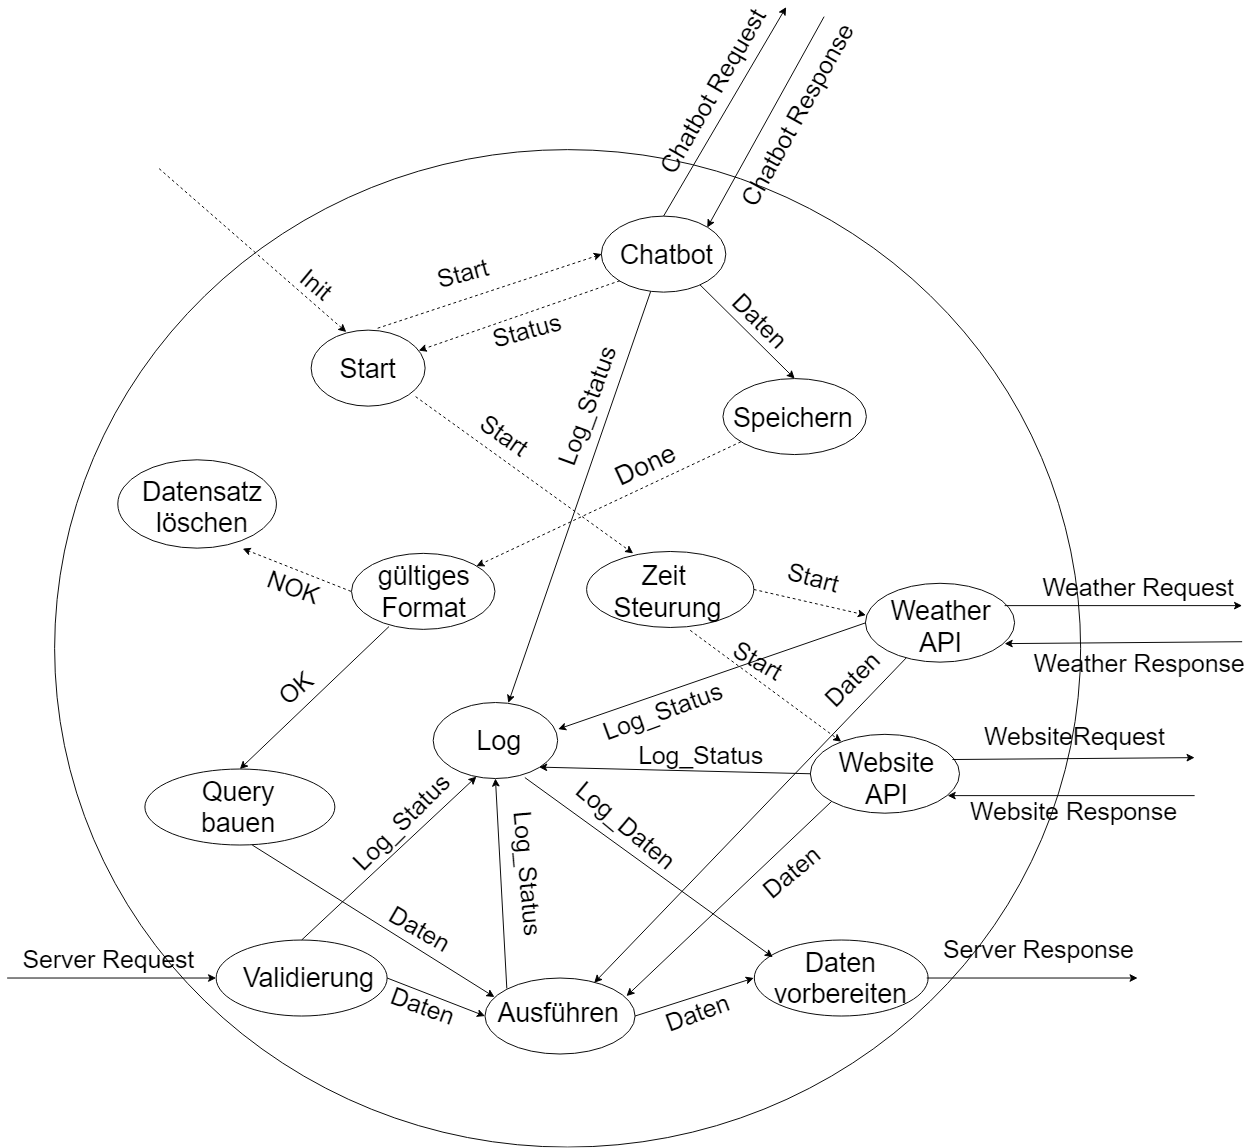
\includegraphics[width=\linewidth]{./figures/server.png}
	\caption{Server}
	\label{fig:erd}
\end{figure}
\subsection{Konfiguration von Raspberry PI Server}
\begin{itemize}
	\item Zuerst wurde ein Image daraufgespielt, die das Betriebssystem von Raspberry PI beinhaltet
\end{itemize}
\begin{itemize}
	\item Danach wurden die folgenden gebrauchten Paketen installiert: git, vim, apache2, python-pip, telepot, php php-mbstring, mariadb-server php-mysql, phpmyadmin
\end{itemize}
\begin{itemize}
	\item In der Konfigurationsdatei wurde die IP-Adresse von dem Raspberry PI angelegt
\end{itemize}
\begin{itemize}
	\item Der nächste Schritt war die Erstellung der Datenbank und der dazugehörigen Tabellen
\end{itemize}
\begin{itemize}
	\item Dann wurden die Benutzer angelegt und die Rechte vergeben
\end{itemize}
\begin{itemize}
	\item Als letztens wurde SSH\footnote{Secure Shell}\nomenclature{SSH}{Secure Shell} aktiviert, damit eine sichere Verbindung zu diesem Server von einem externen Gerät ermöglicht werden kann
\end{itemize}
\subsection{Datenbank}
\begin{itemize}
	\item Zuerst wurde ein ER\footnote{Entity Relationship}\nomenclature{ER}{Entity Relationship} Diagramm mit Papier gezeichnet. Das Ziel war die richtige Erstellung der benötigten Tabellen. Die Tabellen wurden mit den Spalten und ihren Datentypen erstellt. Es wurden auch die Kardinalitäten dazwischen gezeichnet. Die erstellten Tabellen waren:
	
	\begin{itemize}
		\item Supplierplan
	\end{itemize}
    \begin{itemize}
    	\item Stundenplan
    \end{itemize}
    \begin{itemize}
    	\item Wetterdaten
    \end{itemize}
    \begin{itemize}
	\item Chatbot Users
    \end{itemize}	
\end{itemize}
\begin{itemize}
	\item Basierend auf das ER Diagramm wurden dann die Tabellen mit phpmyadmin erstellt
\end{itemize}
\begin{itemize}
	\item Dann sind für alle Tabellen mit MySQL Workbench die entsprechenden gespeicherten Prozeduren erstellt 
\end{itemize}	
\begin{figure}[ht]	
	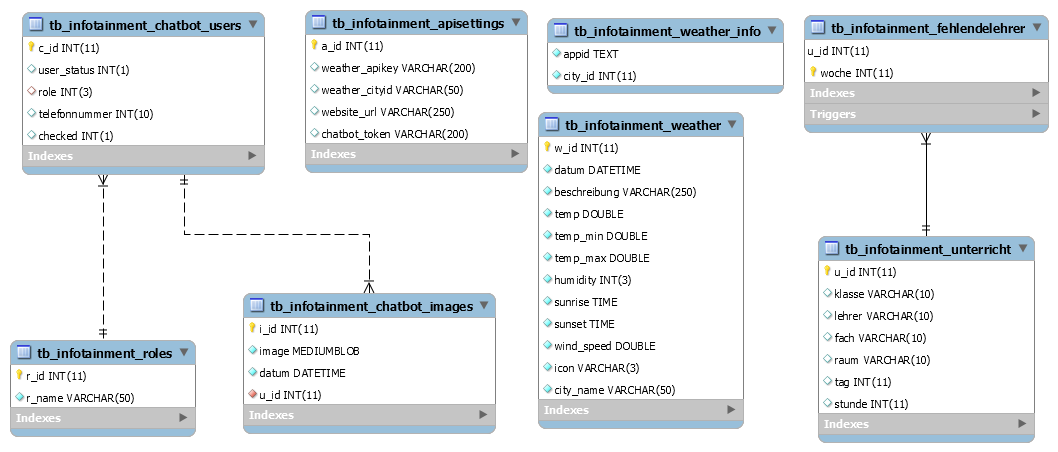
\includegraphics[width=\linewidth]{./figures/erd_irena.png}
	\caption{ERD}
	\label{fig:erd}
\end{figure}
\subsection{SSL Verschlüsselung}
Es wurde ein SSL Zertifikat für den Apache HTTP Server eingerichtet 
\begin{itemize}
	\item Zuerst wurde das SSL Modul für Apache aktiviert
\end{itemize}
\begin{itemize}
	\item Danach wurde das SSL Zertifikat erstellt. 
\end{itemize}
\begin{itemize}
	\item Nach der Erstellung des SSL Zertifikats werden einige Eingaben geschickt, die erfüllt werden sollen. 
\end{itemize}
\begin{itemize}
	\item Danach wurde die Datei /etc/apache2/sites-available/default-ssl.conf geöffnet.
\end{itemize}
\begin{itemize}
	\item Unter der Zeile, wo SSL Engine On steht, wurden die erstellten Zertifikatdateien zugefügt
\end{itemize}
\begin{itemize}
	\item Danach wurde der Virtuellhost mit SSL aktiviert. 
\end{itemize}
\begin{itemize}
	\item Es wurde ein System reboot gemacht und der Apache Server noch einmal gestartet \cite{50_SSS}
\end{itemize}

\subsection{Wetterdaten}
\begin{itemize}
	\item Als erster Schritt erfolgte die Registrierung bei openweathermap.org 
\end{itemize}
\begin{itemize}
	\item 	Danach wurde ein API Key bekannt gegeben, mit dem die API Call gemacht werden kann
\end{itemize}
\begin{itemize}
	\item Die Antwort von API Call wird im JSON-Format gegeben
\end{itemize}
\begin{itemize}
	\item Danach erfolgt die Speicherung der bestimmten Parameter, die von dem API CALL kommen, in der Datenbank
\end{itemize}
\begin{itemize}
	\item Als letztens werden mithilfe von PHP die in der Datenbank gespeicherten Parameter aufgerufen und auf dem Bildschirm angezeigt
\end{itemize}
\subsection{Anzeige}	
\subsection{Chatbot}
In diesem Unterkapitel wird der Chatbot erklärt und dessen Umsetzung auch.
\subsection{Chatbot Einrichtung:}
\begin{itemize}
	\item Zuerst wurde die Telegram Applikation auf dem Handy heruntergeladen
\end{itemize}
\begin{itemize}
	\item Als nächstes wurde es nach einem Benutzer mit der Name Botfather gesucht. Der Botfather ist der Verwalter von Bots und ist für die Einrichtung des Chatbots zuständig.
\end{itemize}
\begin{itemize}
	\item Danach wurde zum Botfather eine Anfrage geschickt, um einen neuen Bot zu erstellen. 
\end{itemize}
\begin{itemize}
	\item Der Botfather fragte danach nach, wie das neue Bot genannt wird und was für ein Benutzername es haben wird.  
\end{itemize}
\begin{itemize}
	\item Danach wurde von dem Botfather das Token des neuen Bots bekannt gegeben, mit dem der Bot weiterentwickelt werden kann. 
\end{itemize}
\begin{itemize}
	\item Nach der Durchführung von diesen Schritten, ist der Bot fertig erstellt geworden. Es könnte dann mit dem angegebenen Benutzernamen durchgesucht werden und der entsprechende Chat damit geöffnet werden. 
\end{itemize}
\subsection{Einrichtung des Chatbots in RaspberryPI}
Die Entwicklung und die Programmierung von Chatbot wurde im RaspberryPI Server gemacht. Damit der RaspberryPI mit dem Telegram Bot API verbunden werden kann, sollten im Raspberry PI zwei Paketen installiert werden. Diese Paketen sind telepot und python-pip. Telepot ist die Pakete, die die Verbindung zum Telegram Bot API erstellt und mit einem Python-Framework funktioniert.\cite{50_telegram}
\subsection{Grundlagen für die Umsetzung von Chatbot}
\begin{itemize}
	\item Zuerst wurde ein Python Skript erstellt.
\end{itemize}
\begin{itemize}
	\item Danach wurden die benötigten Modulen für den Python Interpreter importiert.  Der wichtigste davon ist der, der die Schnittstelle zum Telegram Bot API bildet.
\end{itemize}
\begin{itemize}
	\item Der Token, den wir von dem Botfather bekommen haben, wurde in einer Variable gespeichert. Mit diesem Token ist der Zugriff zu dem erstellten Bot möglich. Mit den dargestellten Funktionen sollte die Verbindung zu dem Infotainment Bot erfolgen und gleichzeitig sollte auch getestet ob diese Verbindung überhaupt funktioniert und ob Informationen von dem Bot zurückkommen. 

\end{itemize}
\begin{itemize}
	\item Dann erfolgt die Verbindung zu der Datenbank. Um die Verbindung mit der Datenbank zu ermöglichen, sollte zuerst die MySQL Bibliothek importiert. Das wurde bei dem zweiten Schritt gemacht. 
\end{itemize}
\subsection{Funktionalitäten von Chatbot}
Je nachdem ob die Person, die eine Nachricht zu dem Infotainment Bot schickt, ein Administrator, ein normaler Benutzer oder ein unregistrierter Benutzer ist, werden ihn verschiedene Funktionalitäten angeboten. 
\subsection{Unregistrierte Benutzer:}
Wenn eine Person zum ersten Mal eine Nachricht zum Infotainment Bot schickt, ist er noch nicht in der Datenbank registriert. Der Bot wird ihn fragen ob er registrieren will oder nicht. Die Möglichkeit zur Registrierung erfolgt durch zwei Buttonen, die im Bot integriert werden. Falls der unregistrierte Benutzer Ja druckt, bittet er ihn die Telefonnummer einzugeben. Durch diese Telefonnummer wird dann der Benutzer in der Datenbank gespeichert. Falls nein, wird ihm nur eine Nachricht vom Chatbot zurückgeschickt. 

Die Telefonnummer, die von dem unregistrierten Benutzer eingegeben wird soll nach Inhalt überprüft werden. Wenn der Benutzer z.B Text eingibt, wird das nicht genehmigt und nicht gespeichert. Falls eine Zahl ist, soll es 10 Ziffern lang sein und mit einem vorgelegten Prefix anfangen. Ansonsten wird es nicht genehmigt und der unregistrierter Benutzer kriegt wieder Möglichkeiten vom Chatbot die Nummer richtig zu schreiben. 

Die Informationen über den unregistrierten Benutzer wird der Administrator bekommen. Er soll dann die Genehmigung geben, ob diese Person schon eine Interaktion mit dem Chatbot haben darf oder nicht. 
\subsubsection{Normale Benutzer:}
Die Daten über die normalen Benutzer sind in der Datenbank gespeichert. Diese Benutzer sind von dem Administrator genehmigt. Die Nachrichten, die diese normalen Benutzer zum Chatbot schicken werden nach Inhalt überprüft. Falls sie ein Bild schicken, wird dieses Bild auf die Datenbank gespeichert und auf dem Bildschirm angezeigt. 
Wenn aber der Benutzer eine Nachricht schickt, die kein Bild ist, wird es keine Interaktion mit dem Bot geben, weil dem Bot interessieren die anderen Nachrichtformate nicht.

\subsubsection{Administrator:}
Dem Administrator werden andere Möglichkeiten zur Verfügung gestellt. Er ist in der Lage die normalen und die unregistrierten Benutzer zu sehen. Die werden von der Datenbank selektiert und durch den Bot dargestellt. Dort kann er die Genehmigung für die unregistrierten Benutzer geben. Er kann auch die normalen Benutzer blockieren, wenn sie einmal ein unpassendes Bild geschickt haben. 
\\
\subsubsection{Umsetzung der Funktionalitäten:}
\begin{itemize}
	\item Zuerst wurde ein Query geschrieben, um zu überprüfen ob die Person, die eine Nachricht zum Bot geschrieben hat, schon in der Datenbank registriert ist oder nicht. \\
\end{itemize} 


\begin{lstlisting}[frame=single]
query=("SELECT c_id, role, user_status, checked, telefonnummer 
from  tb_infotainment_system_chatbot_users 
where c_id = %s") %(int(char_id))
count=curs.execute(query)
if count > 0:
	user=curs.fetchone()
\end{lstlisting}
\captionof{lstlisting}{Chatbot 1}
\begin{itemize}
	\item Falls diese Person registriert ist, wird überprüft ob er ein Administrator oder ein normaler Benutzer ist. Falls er ein Administrator ist, werden die Nachrichten, die er zum Chatbot sendet analysiert und die entsprechenden Ergebnisse zurückgeschickt. 
\end{itemize}	
\begin{itemize}
	\item Wenn der Administrator /users zum Bot schreibt, bedeutet dass er die normalen Benutzer sehen will. Es wird ein Query geschrieben, die diese Benutzer aus der Datenbank selektiert. An dem Administrator wird nur die ID des Benutzers geschickt.
\end{itemize}
\begin{lstlisting}[frame=single]
if command == '/users/:
	curs.execute('Select c_id, role, user_status from 
	tb_infotainment_chatbot_users')
	variable1=curs.fetchall()
	for users in variable1:
		bot.sendMessage(chat_id, users[1])
\end{lstlisting}
\captionof{lstlisting}{Chatbot 2}
\begin{itemize}
	\item Wenn der Administrator /SeeUnregisteredUsers zum Chatbot schreibt, bedeutet dass er die unregistrierten Benutzer sehen will. Ihm werden dann die ID und die Telefonnummer von diesen Benutzer zurueckgeschickt. 
\end{itemize}
\begin{lstlisting}[frame=single]
if command == '/see_unregistered_users':
	curs.execute("Select c_id, telefonnummer,
	(row_number() over (order by c_id) 
	from tb_infotainment_chatbot_users where checked=0")
	unconfirmed=curs.fetchall()
	users=""
	for user in unconfirmed:
		users+=(str(user[2])+" "+str(user[0])+
		" "+str(user[1])+"\n")
		bot.sendMessage(chat_id,users)
\end{lstlisting}
\captionof{lstlisting}{Chatbot 3}
\begin{itemize}
	\item Wenn der Administrator /DoNotAccept und eine bestimmte Chat ID zum Chatbot schreibt, bedeutet, dass der einen unregistrierten Benutzer nicht genehmigen will. 
\end{itemize}	
\begin{lstlisting}[frame=single]
DoNotAccept=command.split()
if DoNotAccept[0] == '/DoNotAccept':
	confirmationquery=
	("update tb_infotainment_chatbot_users 
	set checked=2 where c_id = %s") %(int(DoNotAccept[1]))
	curs.execute(confirmationquery)
	conn.commit()
\end{lstlisting}
\captionof{lstlisting}{Chatbot 3}
\begin{itemize}
	\item Der Administrator kann bestimmte Benutzer blockieren, wenn er ‘/Block’ und eine bestimmte Chat ID zum Chatbot schreibt. 
\end{itemize}
\begin{lstlisting}[frame=single]
block=command.split()
if block[0] == '/block':
	updatequery = ("update tb_infotainment_chatbot_users 
	set user_status='0' where c_id = %s") %(int(block[1]))
	curs.execute(updatequery)
	conn.commit()
\end{lstlisting}
\captionof{lstlisting}{Chatbot 4}

\begin{itemize}
	\item Falls ein normaler Benutzer die oberen Befehle probiert, wird der Chatbot ihn eine Nachricht zurückschicken, dass er nicht der Administrator ist.
\end{itemize}
\begin{itemize}
	\item Durch diese Funktion wird überprüft, ob die Person, die den Button Ja gedruckt hat, registriert ist oder nicht. Falls nein bittet Chatbot ihn, die Telefonnummer einzuschreiben.
\end{itemize}
\begin{lstlisting}[frame=single]
def on_callback_query(msg):
query_id, from_id, query_data=
telepot.glance(msg,flavor='callback_query')
bot.answerCallbackQuery(query_id, text='getIt')
if query_data=='press1':
	bot.sendMessage(from_id, text="ok")
	query2=("Select c_id from tb_infotainment_chatbot_users
	 where c_id=%s") %(int(from_id))
	count1=curs.execute(query2)
if count1 > 0:
	bot.sendMessage(from_id, text="Please write your 
	phone number below")
\end{lstlisting}
\captionof{lstlisting}{Chatbot 5}
\begin{itemize}
	\item Danach erfolgt die Überprüfung ob die Telefonnummer richtig eingegeben ist oder nicht. Falls ja, wird diese Person in die Datenbank hinzugefügt. Der wartet aber auf die Genehmigung des Administrators.
\end{itemize}
\begin{lstlisting}[frame=single] 
query3=("insert into tb_infotainment_chatbot_users" \
"(c_id, user_status, role, telefonnummer, checked)"
"VALUES(%s, %s, %s, %s, %s)")
execute=(chat_id,1,555,reply,0)
curs.execute(query3,execute)
conn.commit()
\end{lstlisting}
\captionof{lstlisting}{Chatbot 6} 
\subsection{Konkrete Beispiele mit Bildern} 
In den folgenden Bildern werden die Funktionalitäten des Administrators beim Chatbot dargestellt.
\begin{itemize}
	\item Funktion des Administrators, die Benutzer anzuschauen. Chatbot schickt die Chat ID des Benutzers zurück, die für jeden Benutzer eindeutig ist, und auch die Telefonnummer. Diese Daten sind in der Datenbank gespeichert und werden davon selektiert.
\end{itemize}
\captionsetup{type=figure}
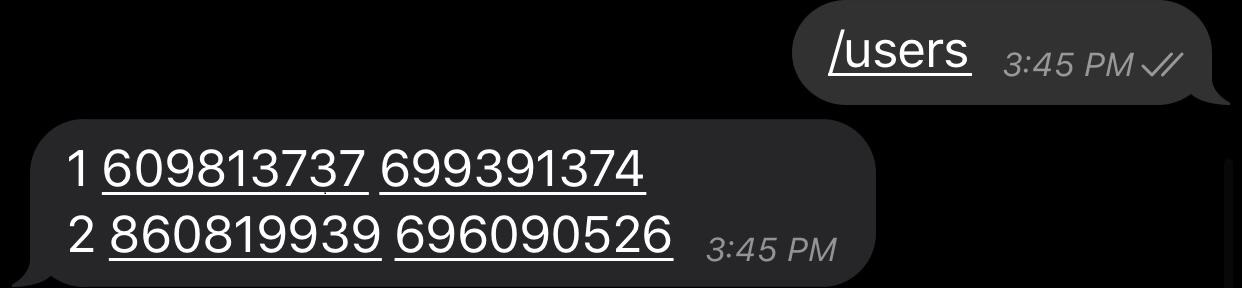
\includegraphics[width=\linewidth]{./figures/chatbotbild88.jpg}
\caption{Auflistung der Chatbot-Benutzer} 
\begin{itemize}
	\item Funktion des Administrators, die unregistrierten Benutzer anzuschauen. Chatbot schickt die Chat ID des Benutzers zurück, die für jeden Benutzer eindeutig ist, und auch die Telefonnummer. Diese Daten sind in der Datenbank gespeichert und werden davon selektiert.
\end{itemize}
\captionsetup{type=figure}
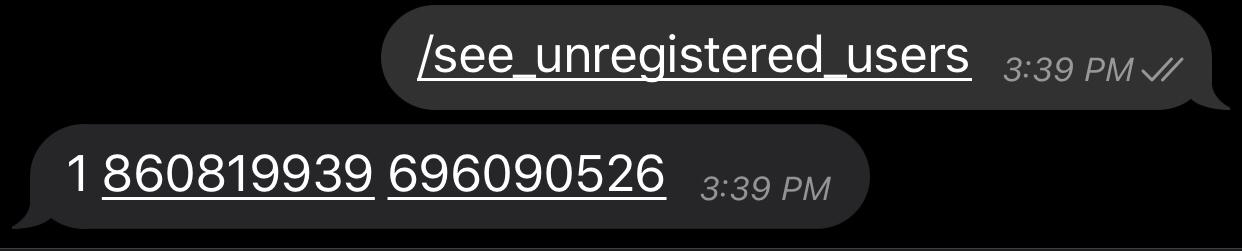
\includegraphics[width=\linewidth]{./figures/chatbotbild9.jpeg}
\caption{Auflistung der unregistrierten Benutzer}
\label{fig:chatbot3}
\begin{itemize}
	\item Funktion des Administrators, die Benutzer zu blockieren. Der Administrator schreibt das einfach das Befehl /block und gibt auch die Chat-ID des Benutzers dazu. Chatbot schickt eine Nachricht zurück.
\end{itemize}
\captionsetup{type=figure}
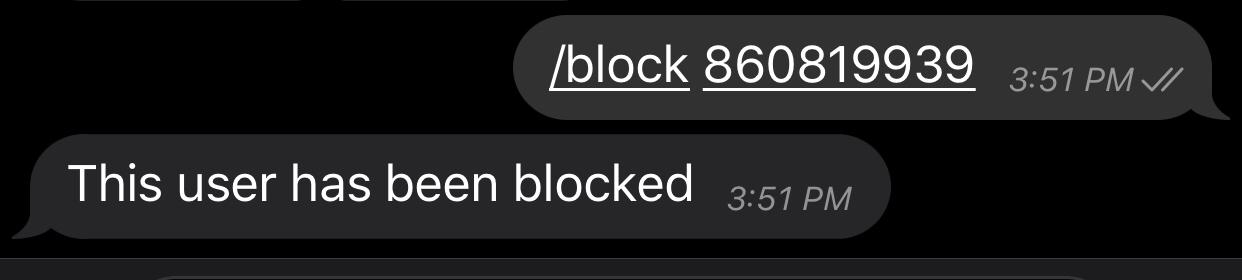
\includegraphics[width=\linewidth]{./figures/chatbotbild11.jpeg}
\caption{Benutzer Blockierung}
\label{fig:chatbot4} 
\newpage
In den folgenden Bildern werden die Funktionalitäten des unregistrierten Benutzer beim Chatbot dargestellt.
\begin{itemize}
	\item Chatbot gibt den Benutzer die Möglichkeit, beim Chatbot zu registrieren. Der Benuter hat zwei Buttons zur Wahl. 
\end{itemize}
\captionsetup{type=figure}
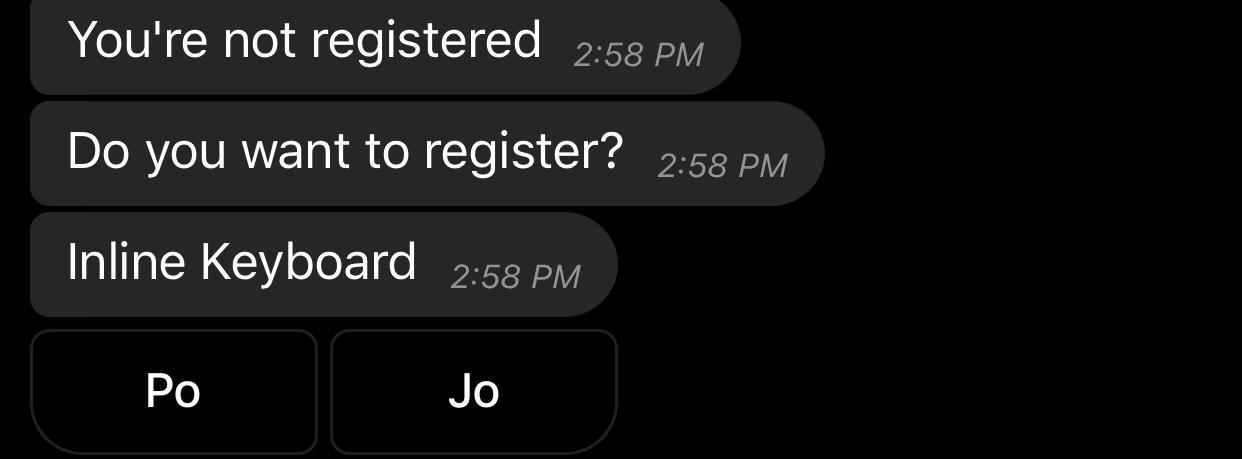
\includegraphics[width=\linewidth]{./figures/chatbotbild.jpeg}
\caption{Registrierung beim Chatbot}
\label{fig:chatbot3}
\begin{itemize}
	\item Wenn der Benutzer Ja klickt, bitten der Chatbot ihn, seine Telefonnummer einzugeben. In diesem Fall hat der Benutzer nur 2 Zahlen eingegeben. Das ist falsch, weil die Telefonnummer 10 Ziffern lang sein soll.
\end{itemize}
\captionsetup{type=figure}
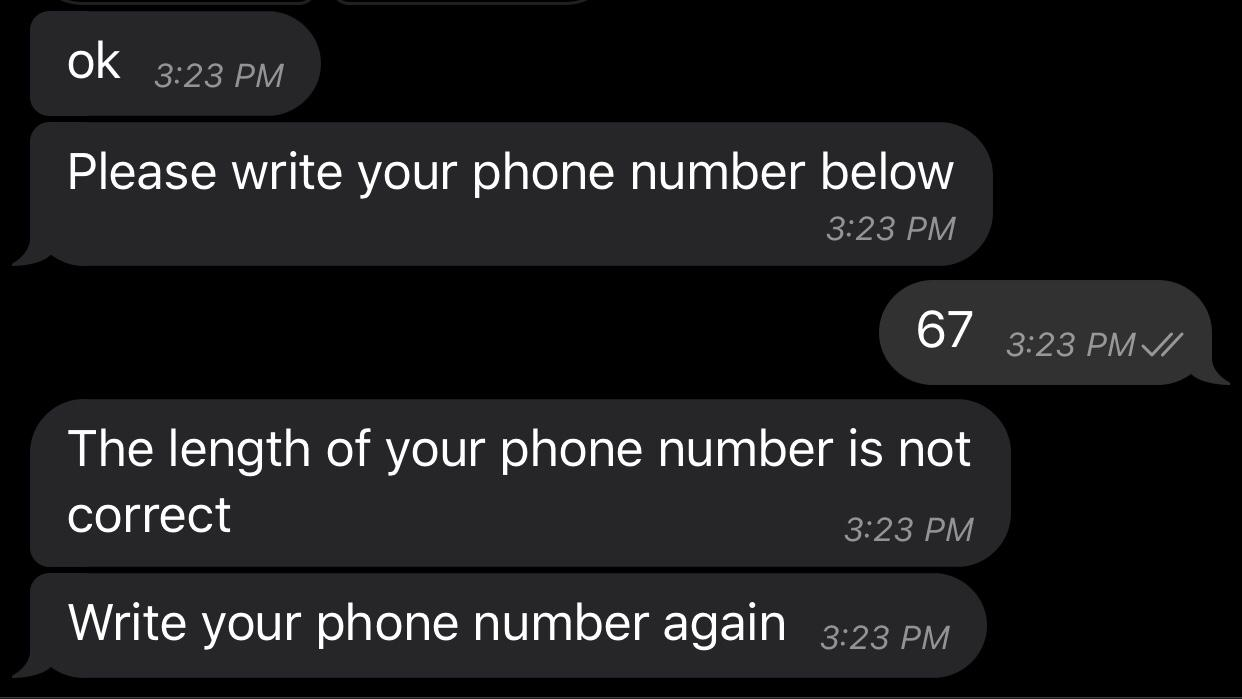
\includegraphics[width=\linewidth]{./figures/chatbotbild2.jpeg}
\caption{Falsche Eingabe des Telefonnummers beim Chatbot}
\label{fig:chatbo73}
\begin{itemize}
	\item Falls der Benutzer statt eine Telefonnummer, ein Text schickt, wird der Chatbot ihm sagen, dass diese Eingabe kein korrektes Format für ein Telefonnummer ist.
\end{itemize}
\captionsetup{type=figure}
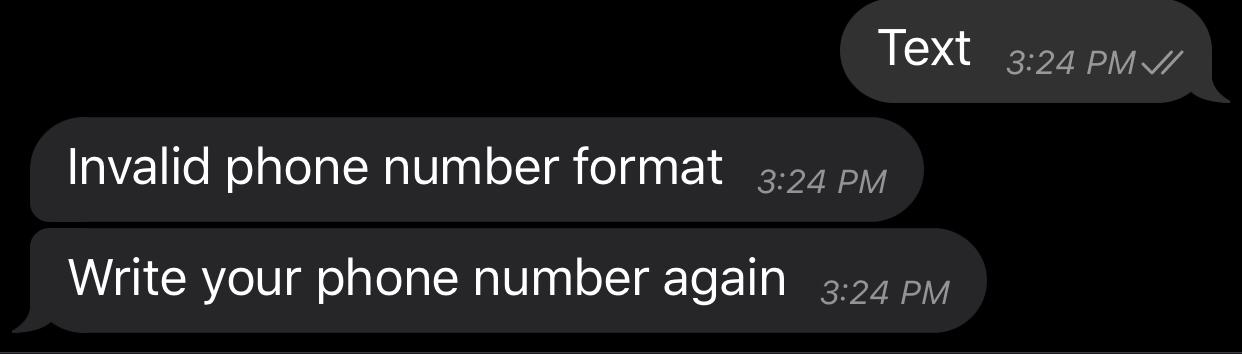
\includegraphics[width=\linewidth]{./figures/chatbotbild5.jpeg}
\caption{Falsches Format des Telefonnummers beim Chatbot}
\label{fig:chatbo73}
\begin{itemize}
	\item Die Telefonnummer soll zu dem Prefix anpassen. Wenn nicht, erkennt der Chatbot das und schikt eine Fehlermeldung zurück.
\end{itemize}
\captionsetup{type=figure}
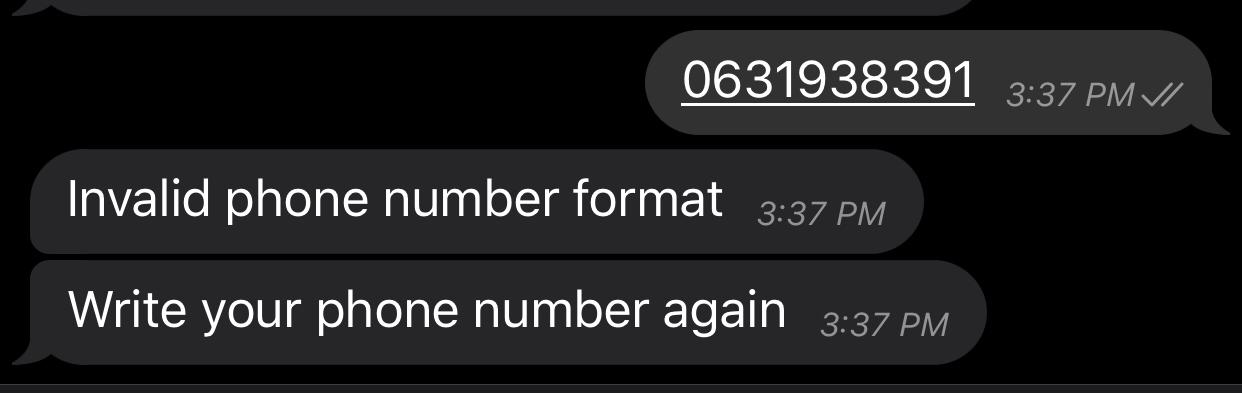
\includegraphics[width=\linewidth]{./figures/chatbotbild6.jpeg}
\caption{Eingabe einer falschen Telefonnummer beim Chatbot}
\label{fig:chatbo53}
\begin{itemize}
	\item Falls der Benutzer die Telefonnummer richtig eingegeben hat, wird ihn eine Nachricht geschickt, dass seine Daten jetzt gespeichert sind. Der Benutzer soll auf die Genehmigung des Administrators warten.
\end{itemize}
\captionsetup{type=figure}
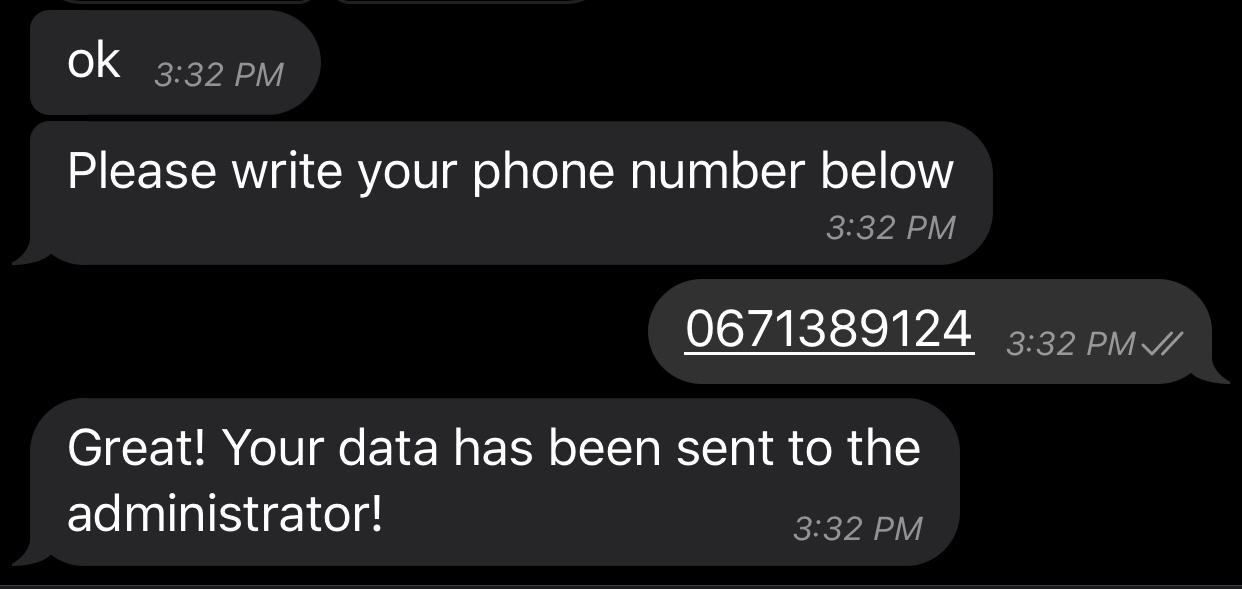
\includegraphics[width=\linewidth]{./figures/chatbotbild4.jpeg}
\caption{Korrekte Eingabe der Telefonnummer beim Chatbot}
\label{fig:chatbo53}
\begin{itemize}
	\item Falls der Benutzer versucht, nachdem er einmal die Telefonnummer eingegeben hat, eine andere Telefonnummer einzugeben, wird der Chatbot ihm eine Nachricht schicken, dass er auf die Genehmigung des Administrators warten soll. Die andere Nachrichte, die später kommen werden nicht berücksichtigt bis der Administrator die Genehmigung gegeben hat.
\end{itemize}
\captionsetup{type=figure}
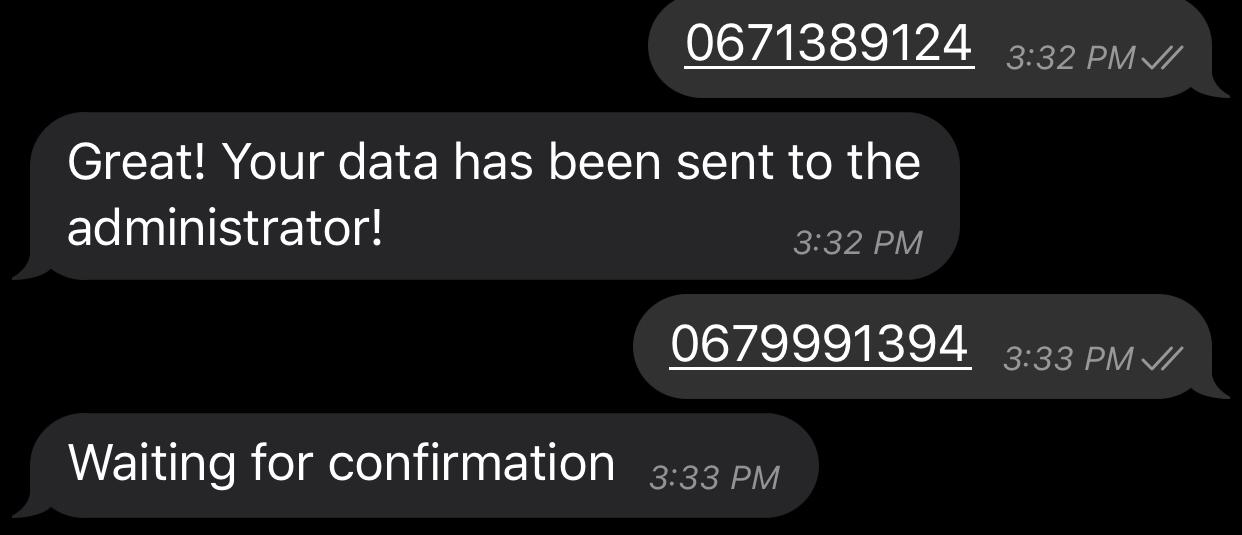
\includegraphics[width=\linewidth]{./figures/chatbotbild7.jpeg}
\caption{Das Warten der Benutzer auf die Administrator Bestätigung}
\label{fig:chatbo53}
In dem folgenden Bild wird die Interaktion eines blockierten Benutzer mit dem Chatbot dargestellt.
\begin{itemize}
	\item Wenn ein Benutzer von dem Administrator blockiert ist und trotzdem versucht eine Nachricht zum Chatbot zu schicken, wird der Chatbot nur eine default Nachricht schicken, falls die vom Benutzer gesendete Nachricht im Textformat ist. Falls dieser Benutzer versucht, ein Bild zu schicken, wird der Chatbot ihm sagen, dass seine Bilder nicht mehr auf dem Bildschirm angezeigt werden.
\end{itemize}
\captionsetup{type=figure}
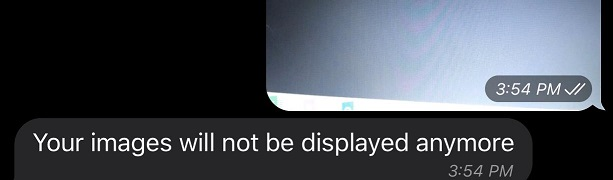
\includegraphics[width=\linewidth]{./figures/catboti.jpg}
\caption{Nachricht von einem blockierten Benutzer}
\label{fig:chatbo53}
\section{Probleme, Herausforderungen und deren Lösung}
\section{Qualitätssicherung, Controlling}
\section{Ergebnisse - Irena Bala}
In diesem Kapitel werden die Ergebnisse der Arbeit zusammengefasst.
\subsection{Implementierung}
Die wichtigsten Ergebnisse der Arbeit sind: 
\nomenclature{$G_e$}{Equivalent Shear Modulus}
\begin{itemize}
	\item Die Implementierung von einem Hauptkomponent der künstlichen Intelligenz wie Chatbot, die das entwickelte System interessanter macht. 
\end{itemize}
\begin{itemize}
	\item Design Vorbereitung für die Anzeige, dass dort die Informationen auf unterschiedliche Weise dargestellt werden können
\end{itemize}
\begin{itemize}
	\item Anlegung einer Datenbank, die die Basis für die Speicherung aller Informationen ist
\end{itemize}
\begin{itemize}
	\item Verwendung von APIs, die die Möglichkeit anbieten Zugriff zu verschiedenen Daten zu haben und als Schnittstelle dienen für die Implementierung von der Komponenten
\end{itemize}
\begin{itemize}
	\item 
	Einrichtung und Anlegung eines Servers, dass auch der Hauptteil des Systems ist und die Basis für die Zusammensetzung aller Komponenten anbietet
\end{itemize}
\begin{itemize}
	\item 
	Integration des Systems, damit alle Komponente mit einander verbinden können
\end{itemize}
\section{Handbuch für die Bedienung}
In diesem Kapitel ist das Handbuch für die Bedienung von Chatbot beschrieben.
\subsection{Beschreibung der Bedienung als User}
Die Bedienung von Chatbot ist eigentlich sehr leicht. Ein normaler Benutzer ist in der Lage, Bilder zum Chatbot zu schicken und die danach in die Datenbank gespeichert und automatisch auf dem Bildschirm angezeigt. \\
Zuerst soll im Handy Telegram Applikation heruntergeladen werden. Danach soll nach dem Benutzername Infotainment gesucht werden. Der Chat mit dem Infotainment Bot wird geöffnet. 
Jeder Benutzer, die eine Interaktion mit Chatbot haben will, soll zuerst registrieren. \\
Sobald der Chatbot eine Nachricht von jemand, der für das erste Mal an ihm etwas schickt, wird der Chatbot ihm fragen ob er registrieren will oder nicht. Die Wahl kommt in Form von 2 Buttons, die die Antworten Ja und Nein beinhalten.\\
Für die Registrierung soll Ja geklickt werden und dann die Telefonnummer für die Registrierung soll auch eingegeben werden. \\
Danach soll gewartet, bis der Administrator die Genehmigung für die neue Registrierung gegeben hat. Sobald der Administrator diese Genehmigung gegeben hat, wird dieser Benutzer eine Nachricht bekommen und nur dann kann er Bilder zum Chatbot schicken, die an dem Bildschirm angezeigt werden.
\subsection{Beschreibung der Bedienung als Administrator}
Der Administrator von Chatbot hat andere Funktionalitäten im Vergleich mit einem Benutzer. 
\begin{itemize}
	\item Wenn die Nachricht /users zum Chatbot geschickt wird, wird dem Administrator eine Liste mit allen Chatbot Benutzer zurückgeschickt.
\end{itemize}
\begin{itemize}
	\item Wenn die Nachricht /SeeUnregisteredUsers zum Chatbot geschickt wird, wird dem Administrator eine Liste mit allen unregistrierten Benutzer zurückgeschickt.
\end{itemize}
\begin{itemize}
	\item Der Administrator kann die Benutzer blockieren durch die folgende Eingabe: /block und die Chat ID von dem Benutzer 
\end{itemize}
\begin{itemize}
	\item Wenn der Administrator eine Registrierung genehmigen will, soll die folgende Eingabe zu dem Chatbot geschickt werden: /Accept und die Chat ID von dem Benutzer
\end{itemize}
\begin{itemize}
	\item Wenn der Administrator eine Registrierung nicht genehmigen will, soll die folgende Eingabe zu dem Chatbot geschickt werden: /DoNotAccept und die Chat ID von dem Benutzer
\end{itemize}
\section{Evaluierung und Resümee}
\subsection{Planung vs Realisierung}
\subsection{Wertschöpfung und Lessons Learned}

	
\label{\docname}

